\newpage
\hypertarget{stringRep vis}{}
\subsection{Implementing toString for \texttt{Box}}
\genHeader

\begin{itemize}

\item[$\blacktriangleright$] Visual SDMs support arbitrary nesting of \emph{for each} story nodes via special guards. In \hyperlink{emptyPartition vis}{Section
5.1} we used the \texttt{[end]} edge guard to terminate a loop. Now we'll use a new guard, the \texttt{[each time]}\define{[each time]} guard, to indicate
control flow that is \emph{nested} and executed for each match. Go ahead and create the SDM for \texttt{Box::toString} until it closely resembles
\Cref{ea:sdm_tostring_1}.

\begin{figure}[htbp]
\begin{center}
  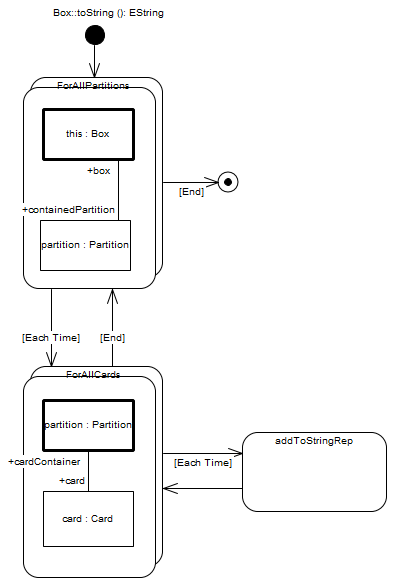
\includegraphics[width=0.8\textwidth]{ea_toStringStart}
  \caption{Control flow with nested loops} 
  \label{ea:sdm_tostring_1}
\end{center}
\end{figure}

\clearpage

\item[$\blacktriangleright$] Knowing \texttt{addToStringRep}'s default node type will not allow it to invoke our helper method, change it
into a \texttt{StatementNode}. Then, analogously to how you established a \emph{MethodCallExpression} for \texttt{grow}, have this node invoke
\texttt{this.addToStringRep(Card)} (\Cref{ea:editStatement1}). 

\vspace{0.5cm}

\item[$\blacktriangleright$] You can see in the \texttt{Method} statement that a \texttt{Card} parameter is required. For this double click on the field below and enter the values like in \Cref{ea:editStatement2}. Now we included \texttt{card} so we may pass the object variable to the method.

\vspace{0.5cm}

\begin{figure}[htbp]
\begin{center}
  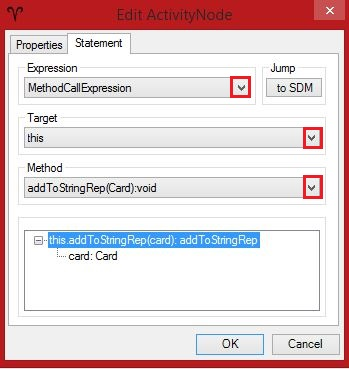
\includegraphics[width=0.5\textwidth]{ea_editStatementNode1}
  \caption{Add a \emph{MethodCallExpression}}
  \label{ea:editStatement1}
\end{center}
\end{figure}

\begin{figure}[htbp]
\begin{center}
  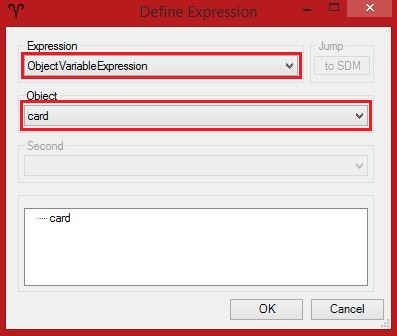
\includegraphics[width=0.5\textwidth]{ea_editStatementNode2}
  \caption{Add a parameter to the \emph{MethodCallExpression}}
  \label{ea:editStatement2}
\end{center}
\end{figure}

\item[$\blacktriangleright$] To complete the SDM, return the final string representation value of the box via an \emph{AttributeValueExpression} in
the stop node (\Cref{ea:toStringStopNode})\define{AttributeValue\-Expression}. This is a new expression type we haven't encountered before. It simply
binds the \texttt{stringRep} attribute of the box (\texttt{this}) to the return value in the stop node


\begin{figure}[htbp]
\begin{center}
  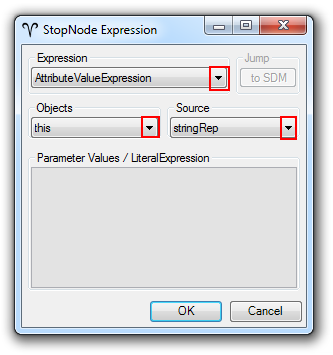
\includegraphics[width=0.45\textwidth]{ea_returnAttributeStopNode}
  \caption{Specify a return value as an \emph{AttributeValueExpression}}
  \label{ea:toStringStopNode}
\end{center}
\end{figure}

\vspace{0.5cm}

\item[$\blacktriangleright$] Take some time to compare and reflect on the complete SDM as depicted in \Cref{ea:sdm_tostringComplete}.  The idea was to
abstract from the actual text representation of the box and model the necessary traversal of the data structure. The helper method \texttt{addToStringRep}
could, for example, build up something totally different.

\vspace{0.5cm}

\item[$\blacktriangleright$] While modelling this SDM, we have seen that \emph{for each} story nodes can be nested, and have used a \emph{MethodCallExpression}
to invoke a void helper method only for its side effects (building up the string representation of the box).

\vspace{0.5cm}

\item[$\blacktriangleright$] As always, save, validate, and build your metamodel in Eclipse.

\begin{figure}[htbp]
\begin{center}
  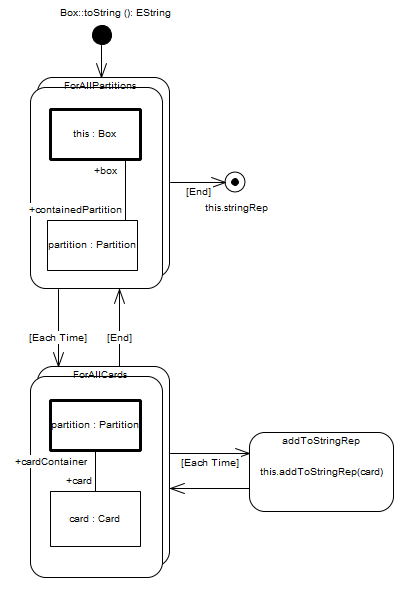
\includegraphics[width=0.8\textwidth]{ea_toStringComplete}
  \caption{The complete SDM for \texttt{Box::toString}}  
  \label{ea:sdm_tostringComplete}
\end{center}
\end{figure}
\FloatBarrier

\end{itemize}
